\subsection{Бифуркционная диаграмма}    

    Для визуализации аттракторов при изменении бифуркационного параметра системы строится бифуркационная диаграмма. Бифуркционная диаграмма для модели (\ref{origin}) при \(\alpha = 1\) представлена на рисунке \ref{bifurcation}.

    \begin{figure}
        \centering
        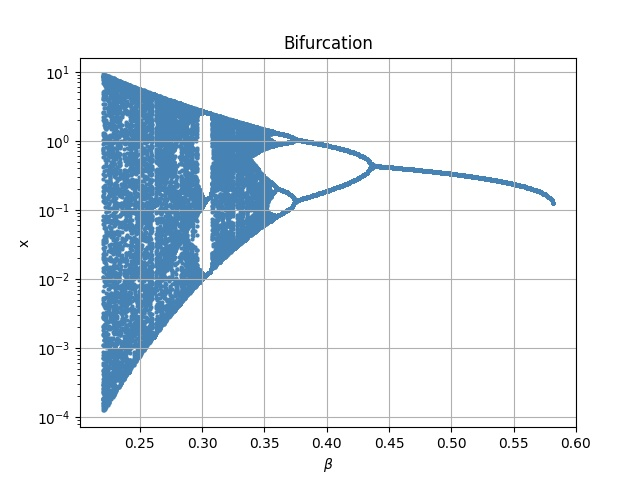
\includegraphics[width=0.9\textwidth]{deterministic/images/bifurcation.jpg}

        \captionsetup{justification=centering}
        \caption{Бифуркационная диаграмма модели (\ref{origin})}
        \label{bifurcation}
    \end{figure}

    Бифуркационная диаграмма показывает в каком диапазоне изменяется численность популяции при конкретном значении параметра \(\beta\).

    Мы видим, что при \(\beta \in [0.44; 0.56]\) --- аттрактором модели (\ref{origin}) является равновесие. Затем происходит удвоение периода и при \(\beta \in [0.37; 0.44]\) видно, что аттрактором является цикл периода 2. На диапазоне \(\beta \in [0.36; 0.37]\) аттрактором является цикл периода 4. И т.д.
        
    Рассмотренные выше интервалы диапазона значений \(\beta\) являются интервалами структурной устойчивости. При дальнейшем уменьшении значения параметра \(\beta\) зона каждого аттрактора становится все меньше и меньше. 
        
    В модели реализуется каскад бифуркаций удвоения периода, приводящий к хаосу \cite[стр. 33]{elementsOfNonlinearDynamic}. Когда наступает хаос, становится невозможным предсказание значения численности популяции в некоторый момент времени при известном начальном значении.
        
    \begin{figure}
        \centering
        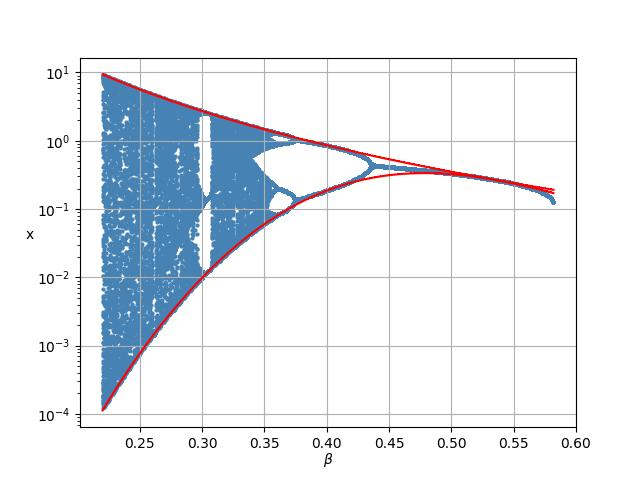
\includegraphics[width=0.9\textwidth]{deterministic/images/bifurcation_chaos.jpg}

        \captionsetup{justification=centering}
        \caption{Бифуркационная диаграмма модели (\ref{origin}) --- синим представлены аттракторы модели, красным --- критические линии }
        \label{bifurcation_chaos}
    \end{figure}
        
    Также на бифуркационную диаграмму можно нанести линии, которые показывают границы хаоса, циклов и части равновесия, опираясь на теорию критических точек \cite{nonsmoothOneDimensionalMapsSomeBasicConceptsAndDefinitions}. Такое можно увидеть на рисунке \ref{bifurcation_chaos}. Также можно заметить, что численность популяции на участке хаоса и циклов не выходит за эти границы.
        
    \begin{figure}
        \centering
        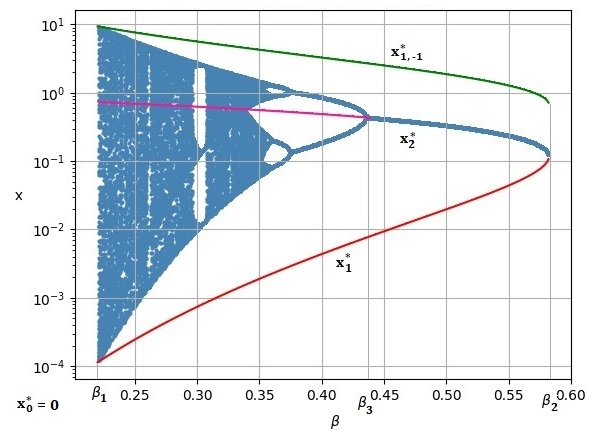
\includegraphics[width=0.8\textwidth]{deterministic/images/bifurcation_attract.jpg}

        \captionsetup{justification=centering}
        \caption{Бифуркационная диаграмма модели (\ref{origin}) с равновесиями и образом равновесия \(x_1^*\) }
        \label{bifurcation_attractor}
    \end{figure}

    На рисунке \ref{bifurcation_attractor} изображена бифуркационная диаграмма, равновесия и прообраз неустойчивого равновесия.

    Заметим, что на интервале от \(\beta_3 \approx 0.44\) до \(\beta_2 \approx 0.58\) устойчивое равновесие является аттрактором \cite{elementsOfNonlinearDynamic}.

    Если начальное значение находится в интервале от \(x_1^*\) до \(x_{1, -1}^*\), то траектория сойдется на равновесие \(x_2^*\). В случае, если траектория начинается за пределом этого интервала, то она сойдется на нулевое равновесие.

    Такую ситуацию мы также можем наблюдать при построении временных рядов. На рисунке \ref{time_series_b_0_56} можно увидеть, что если начальное значение \(x_0 = 0.04\) или \(x_0 = 1.3\), то численность популяции сойдется на нулевое равновесие. Эти значения \(x_0\) лежат вне интервала от \(x_1^*\) до \(x_{1, -1}^*\).

    Рассмотрим временные ряды, которые в качестве начальных значений принимают \(x_0 = 0.06\) и \(x_0 = 0.3\). Такие временные ряды сходятся к значению \(x_2^*\), потому что эти значения лежат в бассейне притяжения.

    Исходя из вышесказанного, можно сделать вывод о том, что равновесия \(x_0^*\) и \(x_2^*\) являются устойчивыми, а равновесие \(x_1^*\) --- неустойчивым.
